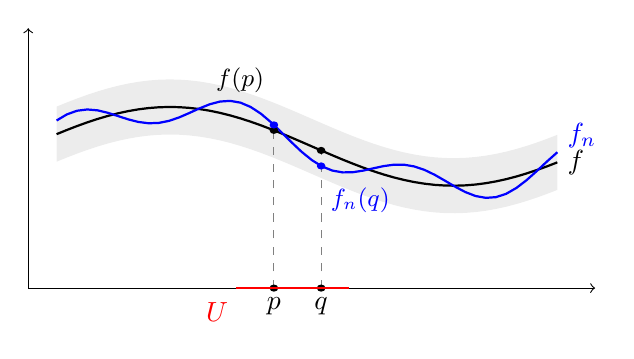
\begin{tikzpicture}[xscale=1.2]
  \draw[->] (0,0) -- (6,0);
  \draw[->] (0,0) -- (0,3.3);
  \fill[gray, opacity=0.15] plot[domain=0.3:5.6, samples=50] (\x, {1.8+0.5*sin(60*\x)+0.35}) -- plot[domain=5.6:0.3, samples=50] (\x, {1.8+0.5*sin(60*\x)-0.35}) -- cycle;
  \draw[thick] plot[domain=0.3:5.6, samples=50] (\x, {1.8+0.5*sin(60*\x)}) node[right] {$f$};
  \draw[blue, thick] plot[domain=0.3:5.6, samples=50] (\x, {1.8+0.5*sin(60*\x)+0.2*sin(200*\x)}) node[right, yshift=6pt] {$f_n$};
  \pgfmathsetmacro{\p}{2.6}
  \pgfmathsetmacro{\q}{3.1}
  \draw[dashed, gray] (\p,0) -- (\p,{1.8+0.5*sin(60*\p)});
  \draw[dashed, gray] (\q,0) -- (\q,{1.8+0.5*sin(60*\q)});
  \fill (\p,{1.8+0.5*sin(60*\p)}) circle (1.3pt);
  \fill[blue] (\p,{1.8+0.5*sin(60*\p)+0.2*sin(200*\p)}) circle (1.3pt);
  \fill (\q,{1.8+0.5*sin(60*\q)}) circle (1.3pt);
  \fill[blue] (\q,{1.8+0.5*sin(60*\q)+0.2*sin(200*\q)}) circle (1.3pt);
  \node[above left] at (\p,{1.8+0.5*sin(60*\p)+0.35}) {\small $f(p)$};
  \node[below right, blue] at (\q,{1.8+0.5*sin(60*\q)-0.35}) {\small $f_n(q)$};
  \fill (\p,0) circle (1.3pt) node[below] {$p$};
  \fill (\q,0) circle (1.3pt) node[below] {$q$};
  \draw[red, thick] (2.2,0) -- (3.4,0);
  \node[red] at (2.0,-0.3) {$U$};
\end{tikzpicture}
